\documentclass{article}

\usepackage[french]{babel}
\usepackage[utf8]{inputenc}
\usepackage{lipsum}
\usepackage{amsmath, amssymb, amsthm, graphicx}
\usepackage{tikz}
\usepackage{multicol}
\usepackage[hidelinks]{hyperref}
\usepackage[numbers,sort]{natbib} % Use natbib for numerical citations in sorted order
\usepackage{caption}
\captionsetup{font=footnotesize}
\usepackage{multirow}
\usepackage{adjustbox}
\usepackage{listings}
\usepackage{float}

\graphicspath{{img/}}
\setlength{\parindent}{0pt}

\newtheorem{theorem}{Théorème}

%%%%%%%%%%%%%%%% Lengths %%%%%%%%%%%%%%%%
\setlength{\textwidth}{16.5cm}
\setlength{\evensidemargin}{-0.5cm}
\setlength{\oddsidemargin}{-0.5cm}
\setlength{\topmargin}{-1.5cm}
\setlength{\textheight}{23cm}


%%%%%%%%%%%%%%%% Variables %%%%%%%%%%%%%%%%
\def\projet{5}
\def\titre{Simulation du comportement de l'air autour d'un profil d'aile d'avion}
\def\groupe{4}
\def\equipe{4}
\def\responsible{Cecile Barrat}
\def\secretary{Melissa Colin}
\def\others{Anas Quatra, Mano Domingo}

\begin{document}

%%%%%%%%%%%%%%%% Header %%%%%%%%%%%%%%%%
\begin{minipage}{0.98\textwidth}
  \vskip 0mm
    { \begin{tabular}{p{7.5cm}}
      {\bfseries \sffamily
        Projet \projet} \\ 
      {\itshape \titre}
    \end{tabular}}
  \hfill 
  \fbox{\begin{tabular}{l}
      {~\hfill \bfseries \sffamily Groupe \groupe\ - Équipe \equipe
        \hfill~} \\[2mm] 
      Responsable : \responsible \\
      Secrétaire : \secretary \\
      Codeurs : \others
    \end{tabular}}
  \vskip 4mm ~

  ~~~\parbox{0.95\textwidth}{\small \textit{Résumé~:} \sffamily 
    Dans ce projet, nous avons étudié le comportement de l'air autour d'un profil d'aile d'avion en utilisant des méthodes d'interpolation et d'intégration. Nous avons utilisé des splines cubiques pour affiner le profil d'aile et différentes méthodes d'intégration pour estimer les longueurs des trajectoires suivies par les particules d'air. Enfin, nous avons calculé la carte de pression en utilisant les résultats de l'interpolation et de l'intégration.}
  \vskip 1mm ~
\end{minipage}

%%%%%%%%%%%%%%%%% TEMPLATE %%%%%%%%%%%%%%%%
\section{Introduction}

L’aérodynamique est un domaine d’étude essentiel dans le domaine de l’aviation. En effet, la portance générée par les ailes d’un avion est un facteur clé pour assurer la sécurité et l’efficacité des vols. La compréhension du comportement de l’air autour des ailes permet de concevoir des avions plus performants et plus sûrs.\\
Dans ce projet, nous allons nous intéresser à la simulation du comportement de l’air autour d’un profil d’aile d’avion. Nous allons utiliser des méthodes d’interpolation et d’intégration pour estimer les longueurs des trajectoires suivies par les particules d’air autour du profil d’aile. Nous allons également calculer la carte de pression en utilisant les résultats de l’interpolation et de l’intégration.\\

\section{Méthodologie}
\begin{minipage}{0.4\textwidth}
  \begin{figure}[H]
    \centering
    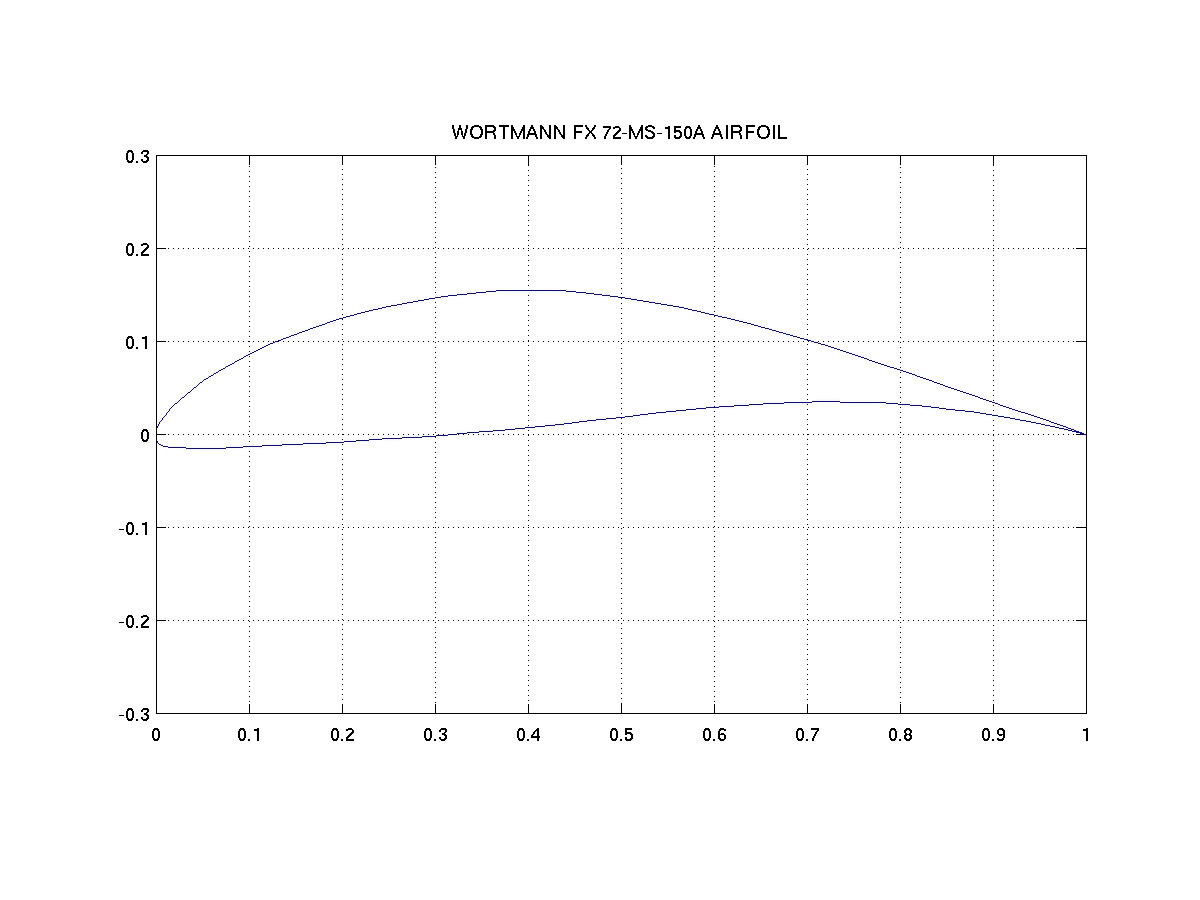
\includegraphics[trim=100 100 100 100, clip, width=\textwidth]{fx72150a.jpg}
    \caption{Modèle d’aile Wortmann FX 72-MS-150A airfoil. Source~\cite{uiuc_fx72150a}}
    \label{fig:airfoil}
  \end{figure}
\end{minipage}
\hfill
\begin{minipage}{0.55\textwidth}
  Pour réaliser ce projet, nous avons choisi d'orienter notre étude sur le modèle d'aile Wortmann FX 72-MS-150A airfoil présenté en figure~\ref{fig:airfoil}. Ce modèle est un profil d’aile conçu pour des planeurs et a été testé sur le Schreder HP-17 en 1973. Il est caractérisé par une faible traînée et une portance élevée~\cite{WikipediaSchrederHP17}. \\ \\
  Le projet s’est déroulé en trois grandes étapes : la première consiste à interpoler les points de la courbe d’un profil d’aile, la seconde consiste à utiliser différentes méthodes d’intégration pour estimer les longueurs des trajectoires suivies par les particules d’air, et la troisième consiste à calculer la carte de pression en utilisant les résultats des deux premières étapes.
\end{minipage}

\subsection{Interpolation par spline cubique}
La première étape de ce projet consiste à affiner le profil d'aile en utilisant des splines cubiques. Celles-ci permettent de représenter la forme de l'aile de manière lisse et continue. \\
Le spline cubique est une fonction $S(x)$ qui interpole un ensemble de points $(x_i, y_i)$ pour $i=0, 1, \ldots, n$ de sorte à ce que $S(x_i) = y_i$ pour chaque $i$. La fonction est continue et possède des dérivées continues jusqu'à l'ordre 2 sur l'intervalle $[x_0, x_n]$.
La spline cubique est une fonction par morceaux, c'est-à-dire qu'elle est définie par plusieurs segments de polynômes cubiques. Chaque segment est défini sur un intervalle $[x_i, x_{i+1}]$ et est relié aux segments adjacents par des conditions de continuité et de dérivabilité. \\ \\
Pour l'implémenter, nous avons appliqué l'algorithme présenté dans le chapitre 3 du livre de \textit{Numerical Recipes}~\cite{press1992numerical}. 
\\
Pour les extrémités, nous avons utiliser des dérivées naturelles (c'est-à-dire les dérivées qui sont nulles aux extrémités de l'intervalle). L'impact de leur valeur est que si les dérivées ne sont pas correctes, la courbe interpolée peut ne pas être lisse ou peut avoir des singularités.\\ \\
Nous l'avons ensuite validé par des tests sur des fonctions connues, telles que $f(x)=x^2$, $f(x)=x^3$ et $f(x)=x^3+2x^2+3x+5$.\\ \\
Pour visualiser le résultat de l'interpolation, nous avons ensuite affiché la courbe d'interpolation avec les points d'origine dans le cas de notre aile d'avion. Nous avons également affiché l'évolution de l'erreur d'interpolation en fonction du nombre de points d'origine. L'erreur est définie comme étant la norme infinie des différences absolues entre les valeurs interpolées et les valeurs exactes, soit $\epsilon = \|S(x) - f(x)\|_{\infty}$.

\subsection{Intégration pour l'estimation des longueurs}
La seconde étape de ce projet consiste à estimer les longueurs des trajectoires suivies par les particules d'air autour du profil d'aile. Pour cela, nous avons utilisé différentes méthodes d'intégration numérique afin de pouvoir sélectionner la plus précise et rapide dans notre contexte. Nous avons choisi de tester les méthodes des rectangles à gauche et à droite, la méthode du point milieu, des trapèzes et de Simpson.\\
\begin{itemize}
  \item[$\bullet$] La méthode des rectangles consiste à approximer l'intégrale d'une fonction en divisant l'intervalle d'intégration en $n$ sous-intervalles de largeur $\Delta x$, représentés par des rectangles construits à partir du point minimal $x$ de l'intervalle (rectangles gauches), ou bien du point maximal $x$ de l'intervalle (rectangles droits).
  \item[$\bullet$] La méthode des trapèzes consiste à réaliser une moyenne des aires de la méthode des rectangles gauches et droits. Cela revient à approximer l'intervalle d'intégration en $n$ sous-intervalles qui approximent la fonction par des fonctions affines. L'aire sous la courbe des fonctions affines est assimilable à celle d'un trapèze.
  \item[$\bullet$] La méthode du point milieu (ou médian) consiste à approximer l'intégrale d'une fonction en divisant l'intervalle d'intégration en $n$ sous-intervalles de largeur $\Delta x$. Dans ces sous-intervalles, nous construisons des rectangles de largeurs $\Delta x$ et de hauteurs $f(x_i)$, où $x_i$ est le point médian de chaque sous-intervalle. L'aire sous la courbe est alors approximée par la somme des aires de ces rectangles.
  \item[$\bullet$] La méthode de Simpson combine les méthodes des trapèzes et du point milieu pour obtenir une approximation plus précise.
  Elle consiste à diviser l'intervalle d'intégration en $n$ sous-intervalles approximés par des polynômes de degré 2.\\
\end{itemize}

De plus, pour estimer l'intégrale d'une fonction avec une précision donnée $\epsilon$, nous avons utilisé la stratégie du doublement de pas. Le principe consiste à calculer successivement l'intégrale en subdivisant l'intervalle $[a,b]$ en un nombre croissant de sous-intervalles, doublé (ou triplé pour la méthode du point milieu) à chaque itération ($n \rightarrow 2n$). À chaque étape, la nouvelle approximation est comparée à celle obtenue précédemment. Si la différence entre les deux devient inférieure à $\epsilon$, l'algorithme s'arrête.\\
Cette méthode permet d’atteindre progressivement une précision voulue, en limitant le nombre de calculs effectués. Elle est particulièrement utile pour éviter de choisir arbitrairement un grand nombre de points d'intégration dès le départ. De plus, elle permet parfois de réutiliser les valeurs déjà évaluées de la fonction pour réduire les coûts de calcul. Le principe est adapté pour toutes les méthodes testées, avec un facteur de subdivision et des sommes évaluées en des points spécifiques. \\ \\
Nous avons implémenté et testé l'ensemble de ces méthodes sur des fonctions et intervalles connus. Puis nous avons comparé la vitesse de convergence de chacune d'entre elles en traçant l'erreur du résultat à chaque itération. L'erreur est définie comme étant la différence absolue entre les valeurs intégrées et les valeurs exactes, soit $\epsilon = \|I - I_{exact}\|$. Nous avons tracé cette convergence sur une fonction de degré 1, 2 et 3, ainsi que sur une fonction circulaire. 

\subsection{Calcul de la carte de pression}
Finalement, nous avons utilisé les résultats de l'interpolation et de l'intégration pour calculer la carte de pression autour du profil d'aile.
Tout d'abord, nous avons représenté le flux laminaire autour de l'aile en appliquant la formule 
$y = f_{\lambda}(x) = (1 - \lambda) f(x) + \lambda \times 3h_{\text{max/min}} \quad \forall \lambda \in [0, 1]$ afin de générer deux familles de courbes représentant respectivement le flux laminaire au-dessus de l'aile (en utilisant $h_{\text{max}}$) et en dessous de l'aile (en utilisant $h_{\text{min}}$). $h_{\text{min}}$ et $h_{\text{max}}$ sont les hauteurs minimales et maximales de l'aile, récupérées sur l'ensemble des points interpolés. \\ \\
Nous avons ensuite pu calculer la carte de pression, celle-ci est donnée par $P = P_s + P_d$ où  $P_s$ est la pression statique et $P_d$ la pression dynamique telle que $P_d = \frac{1}{2} \rho v^2$. $\rho$ étant la densité de l'air et $v$ est la vitesse de l'air. \\
Pour simplifier cette formule, nous avons posé les hypothèses suivantes~:
\begin{enumerate}
  \item Nous avons considéré que la pression est constante entre chaque courbe des familles de flux laminaire.
  \item Nous avons considéré que la densité de l'air est constante et égale à 1 kg/m³, ce qui correspond approximativement à la densité de l'air à 2000 m d'altitude à environ 0°C.
  \item Nous avons considéré que l'air met le même temps $T$ pour traverser la zone qui sépare l'avant de l'arrière de l'aile, quelle que soit la tranche représentée par les courbes de flux laminaire. Par commodité, nous poserons ce temps à $T=1s$. Ainsi, la vitesse de l'air est donnée par la formule $v = \frac{L}{T}$, où $L$ est la longueur de la courbe de flux laminaire. Comme $T=1$, $v=L$.
  \item Nous avons considéré que $P_s$ était négligeable devant $P_d$. Nous l'avons donc retiré de l'équation.
  \item Nous avons supposé que l'air était perturbé entre $3\times h_{\text{max}}$ et $3\times h_{\text{min}}$. En dehors de cette zone, la pression est considérée comme étant 1/2 de la pression atmosphérique étant donné $L = 1$.\\
\end{enumerate}
Nous obtenons alors grâce aux hypothèses précédentes $P = \frac{1}{2} \times \rho \times L^2$.\\ \\
Pour calculer la vitesse de l'air, nous avions besoin de la longueur de chaque courbe de flux laminaire. Pour réaliser cette opération, nous appliquons $L = \int_{0}^{B} \sqrt{1 + (f'(x))^2} dx$. Ici $B$ est la borne maximale du graphe, à savoir $1$, et $f'$ la dérivée de la fonction représentée par la courbe de flux laminaire. Pour intégrer, nous avons utilisé la méthode de Simpson, qui est la plus précise et rapide dans notre cas (la raison de ce choix sera développée dans la section~\ref{sec:affinage}). \\
Enfin, nous avons calculé la pression associée à chaque inter-courbe du flux laminaire puis nous les avons représentées sur un graphique en 2D.
\section{Résultats et discussions}
Dans cette section, nous allons présenter les résultats obtenus lors de la réalisation de ce projet. Nous allons d'abord présenter les résultats de l'interpolation par spline cubique, puis ceux de l'affinage du profil d'aile et enfin ceux du calcul de la carte de pression.

\subsection{Interpolation par spline cubique}
\begin{minipage}{0.45\textwidth}
  L'interpolation par spline cubique a été réalisée avec succès. Nous avons pu obtenir une courbe lisse et continue qui interpole les points d'origine du profil d'aile. \\ \\
  La figure~\ref{fig:spline} montre le résultat de l'interpolation avec les points d'origine en rouge et vert et la courbe interpolée en bleu. Cette courbe est très proche de la courbe d'origine présentée en figure~\ref{fig:airfoil}, ce qui montre que notre méthode d'interpolation est efficace. 
\end{minipage}
\hfill
\hfill
\begin{minipage}{0.5\textwidth}
  \begin{figure}[H]
    \centering
    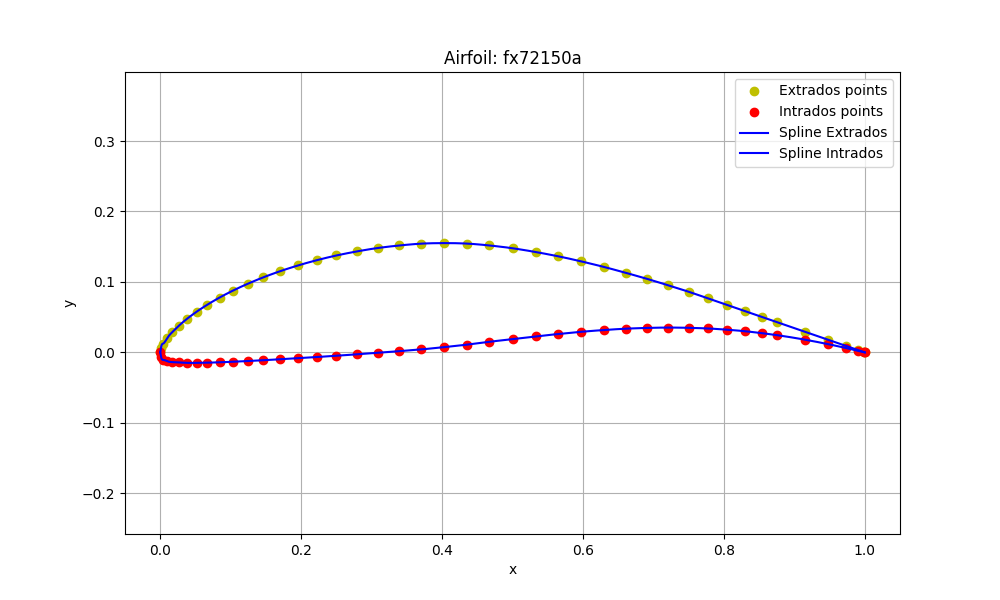
\includegraphics[trim=45 20 70 50, clip, width=\textwidth]{spline.png}
    \caption{Résultat de l'interpolation par spline cubique.}
    \label{fig:spline}
  \end{figure}
  \hspace{0.25cm}
\end{minipage}
Nous avons également tracé l'erreur d'interpolation en fonction du nombre de points d'origine sur différentes fonctions, comme montré dans la figure~\ref{fig:error}. Cette visualisation nous permet dans un premier temps de constater que l'erreur dépend principalement du degré de la fonction à interpoler. En effet, on observe que les fonctions de degré 1 et 2 ont une erreur d'interpolation de l'ordre de $10^{-15}$, tandis que pour les fonctions de degré 3, l'erreur est de l'ordre de $10^{-3}$. De plus, on observe que les fonctions circulaires ont quant à elles une erreur plus faible que les fonctions d'ordre 3 mais plus élevée que les fonctions d'ordre 1 et 2. Néanmoins, elles décroissent extrêmement vite en augmentant le nombre de points d'origine contrairement aux fonctions d'ordre 1 et 2 qui restent constantes quel que soit le nombre de points d'origine.\\ \\
Ceci s'explique par le fait que les fonctions d'ordre 1 et 2 sont linéaires et quadratiques, ce qui signifie qu'elles peuvent être parfaitement interpolées par une spline cubique. L'erreur visible ici correspond à l'erreur machine. En revanche, les fonctions d'ordre 3 et circulaires ne peuvent pas être parfaitement interpolées par une spline cubique, ce qui explique l'erreur d'interpolation plus élevée bien que légèrement décroissante en fonction du nombre de points d'origine.
\begin{figure}[H]
  \centering
  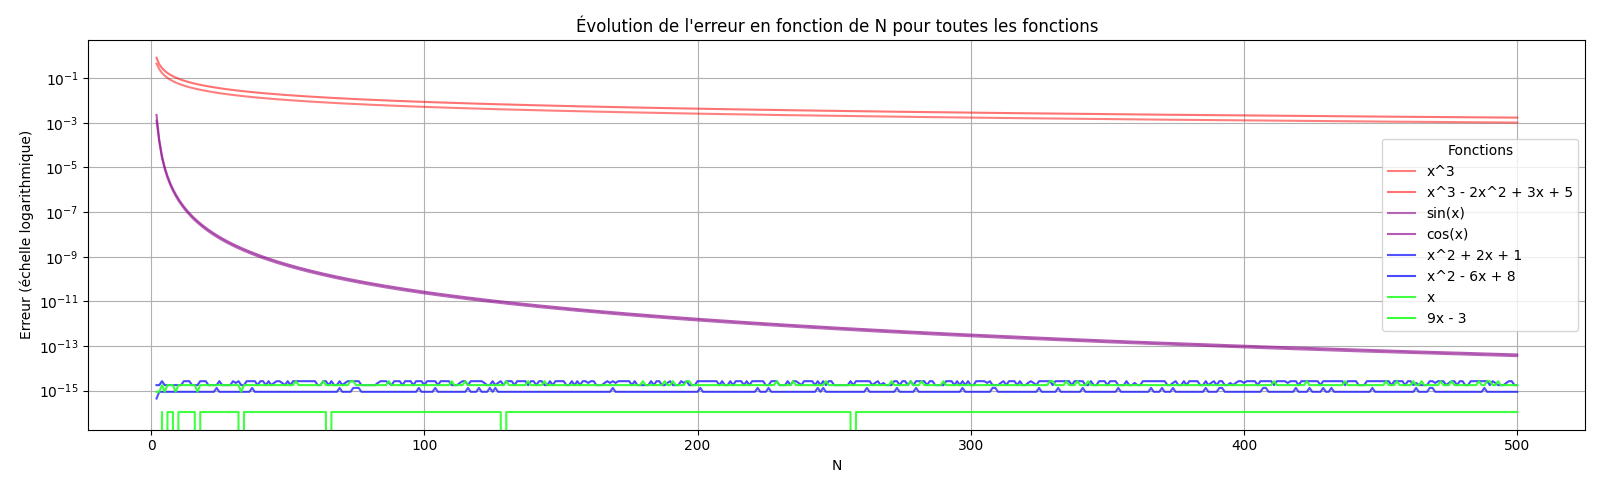
\includegraphics[width=\textwidth]{error_cs.png}
  \caption{Erreur d'interpolation en fonction du nombre de points d'origine N.}
  \label{fig:error}
\end{figure}
Nous avons également observé que l'erreur d'interpolation diminue de manière exponentielle en fonction du nombre de points d'origine. En effet, lorsque le nombre de points d'origine augmente, l'erreur d'interpolation diminue rapidement jusqu'à atteindre une valeur proche de $10^{-15}$ l'erreur machine. Cela montre que notre méthode d'interpolation est très efficace et permet d'obtenir des résultats très précis même avec un nombre limité de points d'origine.

\subsection{Affinage du profil d’aile}
\label{sec:affinage}
En appliquant les différentes méthodes d'intégration, nous avons pu comparer les résultats obtenus avec les valeurs exactes des intégrales. La figure~\ref{fig:integration} montre l'erreur d'intégration en fonction du nombre d'itérations pour chaque méthode sur différentes fonctions.
\begin{figure}[H]
  \centering
  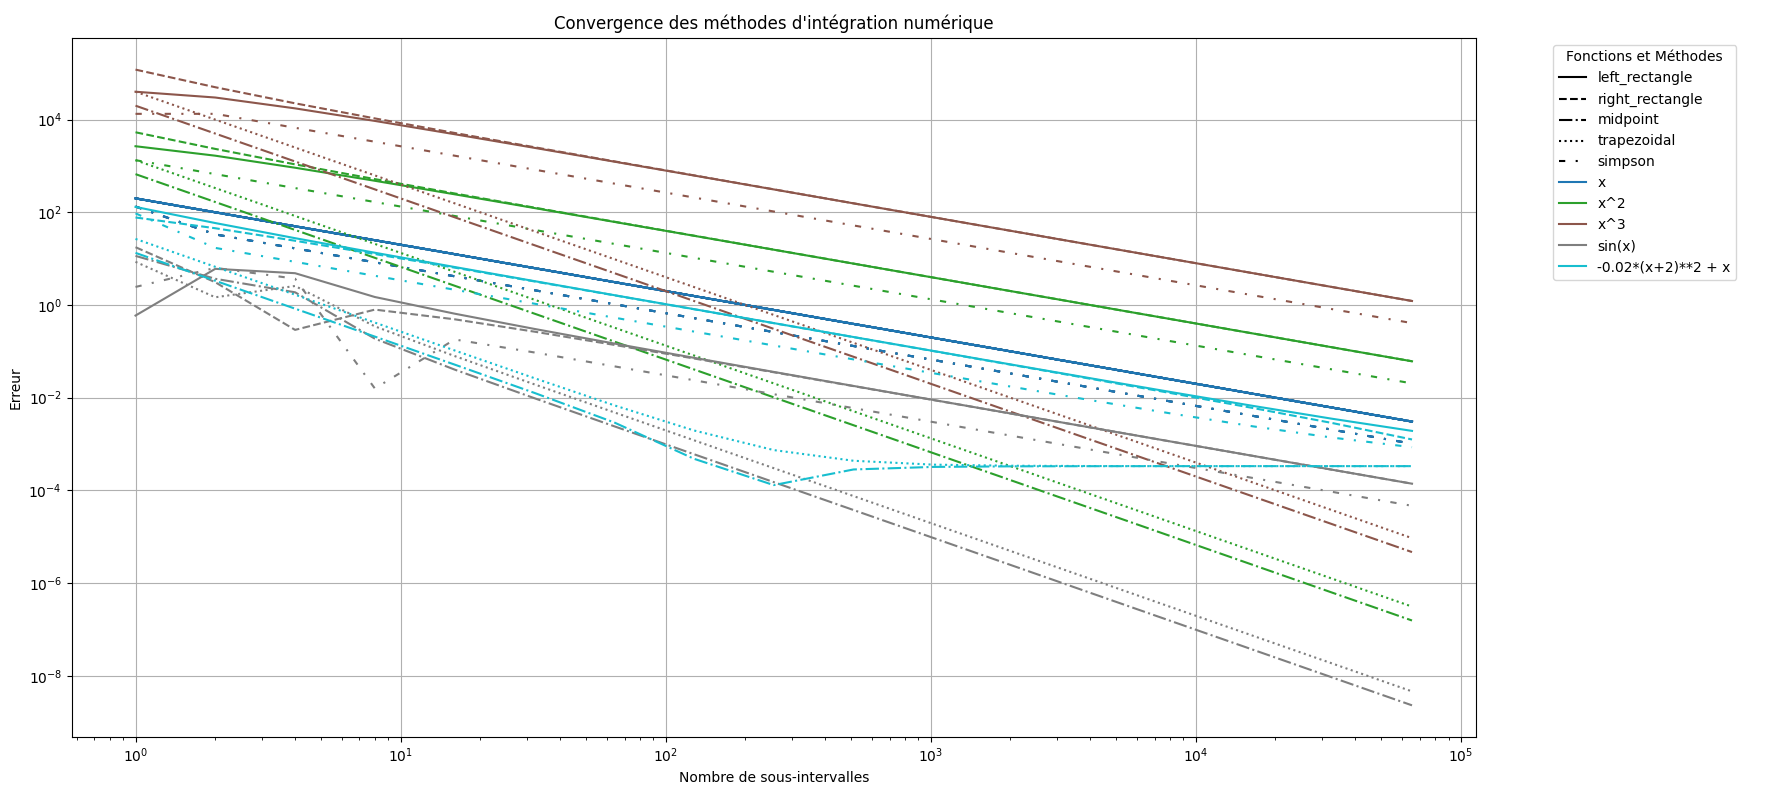
\includegraphics[width=0.9\textwidth]{integration_convergence.png}
  \caption{Erreur d'intégration en fonction du nombre d'itérations N.}
  \label{fig:integration}
\end{figure}
Nous pouvons constater que l'ensemble des méthodes converge vers la valeur exacte de l'intégrale de façon linéaire en général. Cependant, la méthode de Simpson est la plus rapide à converger pour l'ensemble des cas testés. En effet, elle converge beaucoup plus rapidement que les autres méthodes, notamment pour les fonctions d'ordre 3 et circulaires. La méthode des trapèzes est également efficace, mais elle est légèrement moins rapide que la méthode de Simpson. Ceci s'explique par le fait que ces méthodes ne prennent pas en compte la courbure de la fonction, elles sont d'ordre 1 et ne sont donc pas adaptées pour des fonctions plus complexes.\\ \\
Nous pouvons également observer que dans plusieurs cas, au bout d'un certain nombre d'itérations, la méthode de Simpson arrête de converger voire diverge légèrement. Nous pouvons expliquer cela par le fait que lorsque le nombre d'itérations est trop élevé, la méthode de Simpson peut souffrir d'erreurs d'arrondi dues à la représentation numérique des nombres.\\

\subsection{Calcul de la carte de pression}
Nous avons ensuite utilisé les résultats de l'interpolation et de l'intégration pour calculer le profil aérodynamique de l'aile. La figure~\ref{fig:disturbence_curves} montre les courbes de flux laminaire au-dessus et en dessous de l'aile. Nous avons pu observer que le flux laminaire est perturbé entre $3\times h_{\text{max}}$ et $3\times h_{\text{min}}$, ce qui correspond à la zone où la pression est considérée comme étant 1/2 de la pression atmosphérique. En dehors de cette zone, le flux laminaire est considéré comme étant constant.\\
\begin{minipage}{0.5\textwidth}
  \begin{figure}[H]
    \centering
    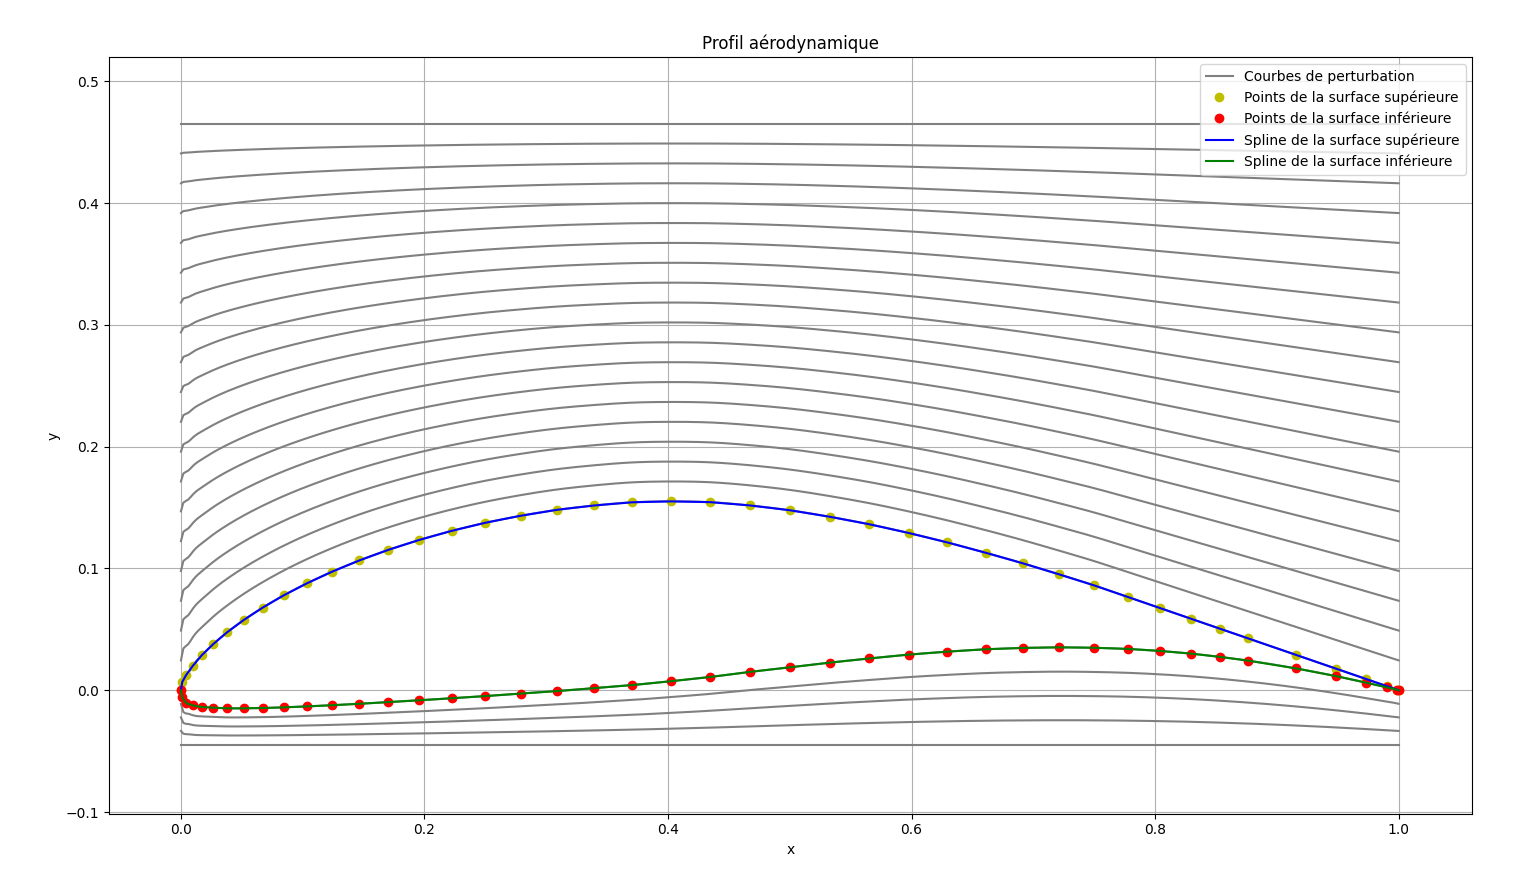
\includegraphics[width=\textwidth]{disturbence_cruves.png}
    \caption{Courbes de flux laminaire au-dessus et en dessous de l'aile.}
    \label{fig:disturbence_curves}
  \end{figure}
\end{minipage}
\hfill
\begin{minipage}{0.5\textwidth}
  \begin{figure}[H]
    \centering
    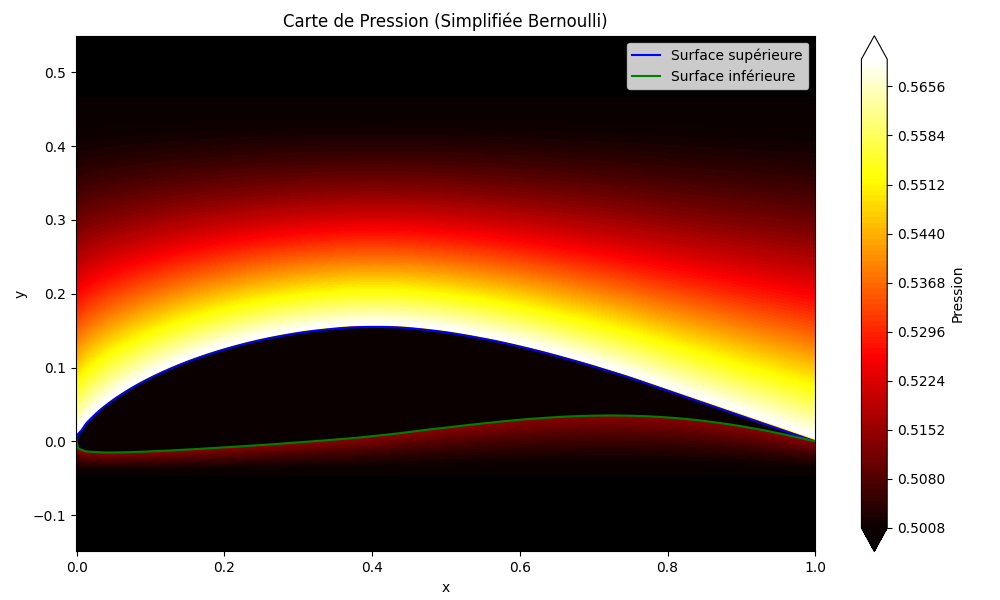
\includegraphics[width=\textwidth]{pressure_map.png}
    \caption{Carte de pression obtenue.}
    \label{fig:pressure_map}
  \end{figure}
\end{minipage}
\phantom{text}\\
Nous avons ensuite calculé la carte de pression en utilisant la formule $P = \frac{1}{2} \times \rho \times L^2$. La figure~\ref{fig:pressure_map} montre la carte de pression obtenue. Nous pouvons observer que la pression est plus élevée au-dessus de l'aile qu'en dessous, ce qui est cohérent avec le concept de portance. En effet, la pression est plus faible au-dessus de l'aile qui permet à l'avion de se maintenir dans les airs durant le vol.

\section{Conclusion et perspectives}
Dans ce projet, nous avons réussi à simuler le comportement de l'air autour d'un profil d'aile d'avion en utilisant des méthodes d'interpolation et d'intégration. Nous avons pu obtenir une courbe lisse et continue qui interpole les points d'origine du profil d'aile. Nous avons également pu estimer les longueurs des trajectoires suivies par les particules d'air autour du profil d'aile en utilisant différentes méthodes d'intégration. Enfin, nous avons pu calculer la carte de pression en utilisant les résultats de l'interpolation et de l'intégration.\\
Nous avons pu observer que la méthode de Simpson est la plus rapide à converger pour l'ensemble des cas testés. Nous avons également pu observer que la pression est plus élevée au-dessus de l'aile qu'en dessous, ce qui est cohérent avec le concept de portance.\\

Pour la suite, nous pourrions envisager d'améliorer notre modèle en prenant en compte d'autres paramètres tels que la viscosité de l'air, les turbulences, ou encore la température. Nous pourrions également envisager d'utiliser des méthodes plus avancées telles que les méthodes de Monte Carlo ou les méthodes de Galerkin pour améliorer la précision de notre simulation. Enfin, nous pourrions envisager d'appliquer notre méthode à d'autres profils d'aile afin de valider notre modèle.




%%%%%%%%%%%%%%%% Bibliography %%%%%%%%%%%%%%%%

\bibliographystyle{plain}
\bibliography{refs}
\end{document}